\documentclass{tufte-book}
\usepackage[utf8]{inputenc}
\usepackage[english]{babel}
\usepackage{amsmath,amsthm,amssymb}
\usepackage{graphicx}
\graphicspath{{../images/}}

\setlength{\parindent}{0pt}

\title{\\ Chemistry \& \\ Materials \\ Science}
\author{Richard Robinson}

\begin{document}
\frontmatter
\maketitle
%\tableofcontents

\setlength{\parindent}{0pt}

\mainmatter


%%%%%%%%%%%%%%%%%%%%%%%%%%%%%%%%%%%%%%%%%%%%%%%%%%%%%%%%%%%%%%%%%%%%%%
% MAIN DOCUMENT
%%%%%%%%%%%%%%%%%%%%%%%%%%%%%%%%%%%%%%%%%%%%%%%%%%%%%%%%%%%%%%%%%%%%%%

\chapter{Introduction}

\section{Stoichiometry}

All stoichiometric equations for quantities may be derived from \begin{equation}
  n_1/v_1 = n_2/v_2
\end{equation}

\begin{marginfigure}
  \begin{center}
    \begin{tabular}{ll}
      moles & $n = m/M = CV$ \\
      atoms & $n_{\mathrm{atoms}} = \rho V N_a / M$ \\
      molarity & $C = mn/MV$ \\
      dilution & $n_1 = n_2$
    \end{tabular} \phantom{mm}
  \end{center}
  \caption[]{Equations for quantities derived from Equation 1.}
\end{marginfigure}

The percentage yield is defined as \begin{equation}
  \text{\% yield} = \frac{\text{actual yield}}{\text{theo. yield}} \times 100 \%
\end{equation}

A crucial aspect in confirming stoichiometric results is using dimensional analysis; that is, using the dimensions of each unit in the equation(s) and confirming the final unit has the proper dimensions.

\section{Bonding}

The total number of orbitals is equal to $n^2$, where $n$ is the principle quantum number, wherein each orbital has a maximum of two electrons.
%
\marginnote{The orbitals are filled in the order of $1s^2 \, 2s^2 \, 2p^6 \, 3s^2 \, 3p^6 \, 4s^2 \, 3d^{10} \, 4p^6 \, 5s^2 \dots$.}
%
This maximum occurs only if all subshells contain one electron originally, known as Hund's rule.

\begin{center}
  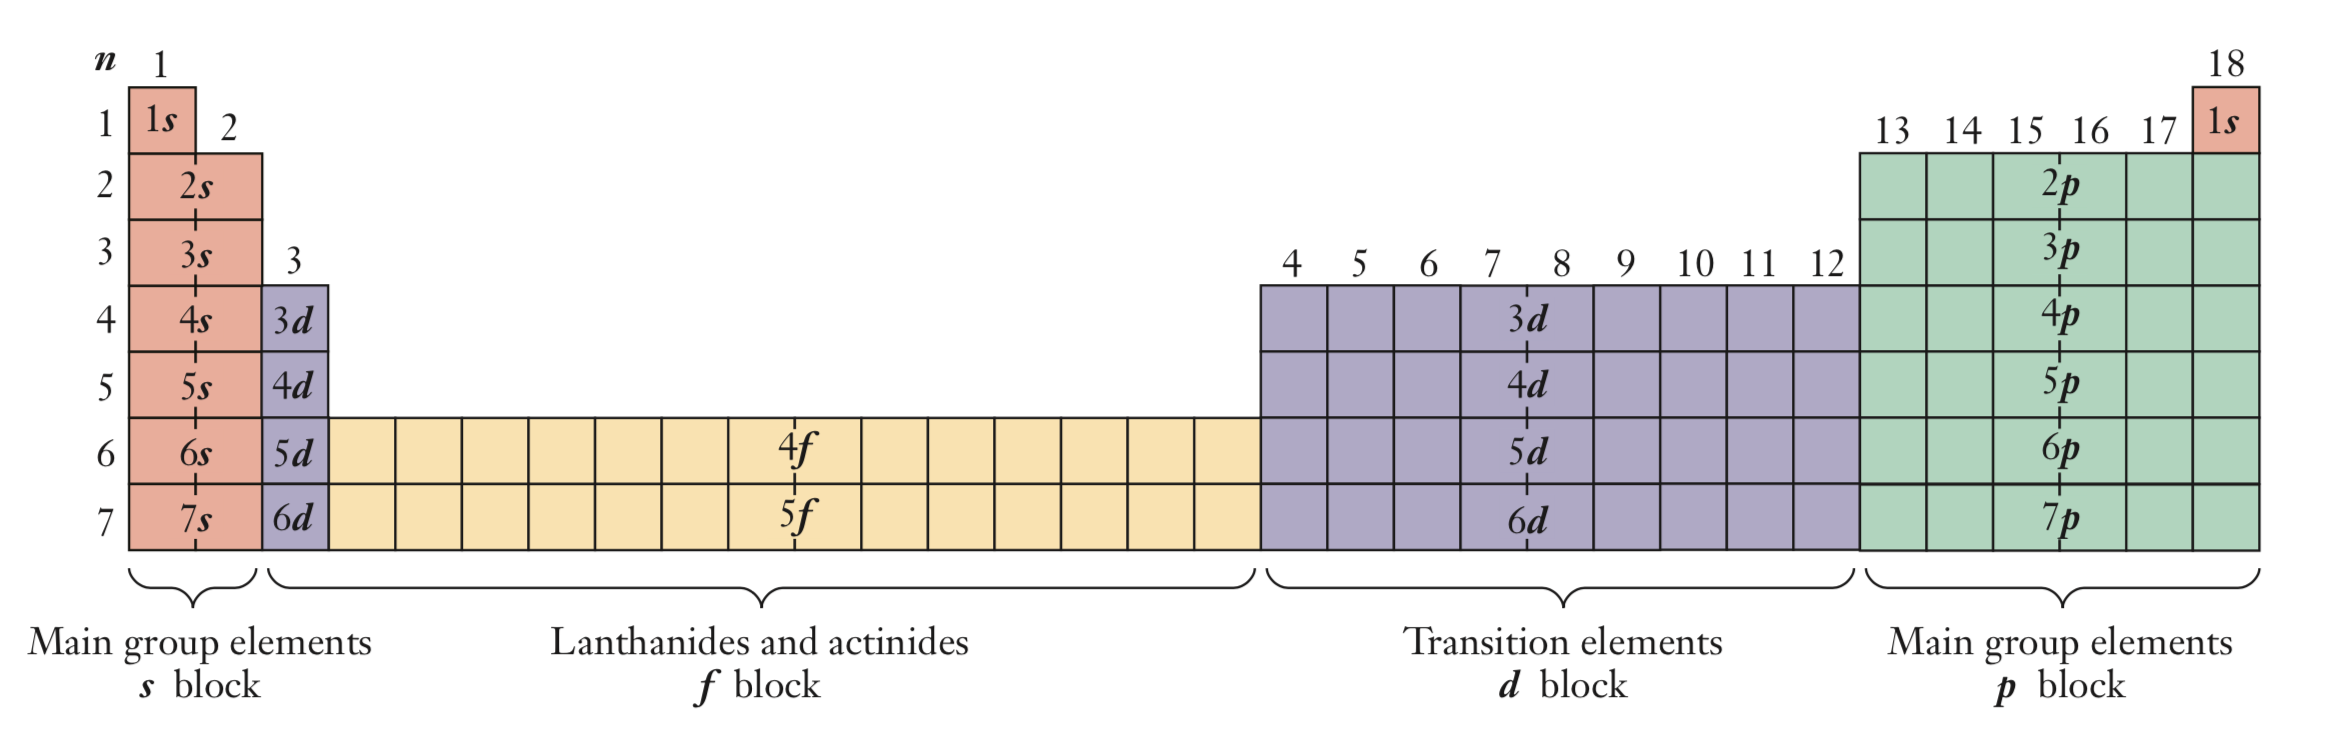
\includegraphics[width=1\textwidth]{table}
\end{center}

The formal charge is given by $q_f = n_v - n_l - \frac{1}{2} n_s$ in which $\sum q_f = 0$.

\marginnote{$n_v$ is the total number of valence electrons; $n_l$ is the number of lone pairs; and $n_s$ is the number of electrons shared in bonds.}

Hybrid orbitals are dependent on molecular geometry, and filled by $sp^3d^2$. The number of orbitals is equal to the number of electron pairs. The number of sigma and pi bonds is equal to \begin{equation}
  n_\sigma = \sum n_\text{all} \quad\text{and}\quad n_\pi = \sum n_\text{dbl} + 2 \sum n_\text{tri}
\end{equation}

\section{Atoms \& Molecules}
Other properties of the periodic table include \begin{itemize}
  \item Atomic size increases toward the bottom left;
  \item Ionization energy and electronegativity increase towards the top right;
\end{itemize}

\begin{marginfigure}
\begin{center}
  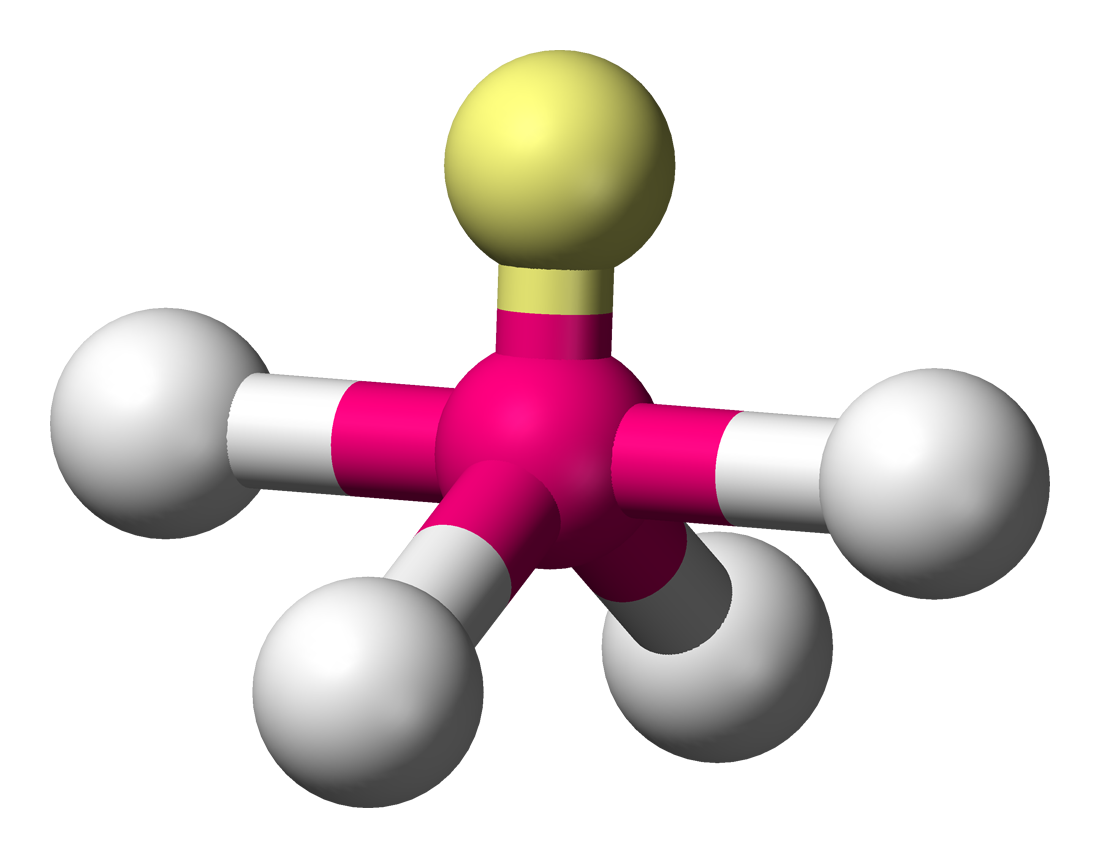
\includegraphics[width=0.5\textwidth]{molecule1} \phantom{mmm}
\end{center}
\caption{The seesaw VSEPR model constructed from a lewis diagram.}
\end{marginfigure}

Lewis dot structures are created via the following algorithm: \begin{enumerate}
  \item Count the total number of valence electrons in the molecule;
  \item Place single bonds between all connected atoms;
  \item Place the remaining valence electrons not accounted for in (2) on individual atoms, specifically as lone pairs whenever possible;
  \item Create multiple bonds as needed for any atoms that do not have a full octet
\end{enumerate}

\chapter{Chemical Equilibrium}

\section{Equilibrium Constants}

A system is said to be at dynamic equilibrium if the rates of both reactions are equal but do not approach zero. For a general chemical reaction, the reaction quotient and equilibrium constant are
\marginnote{A general equilibrium reaction is given by $aA + bB \leftrightharpoons cC + dD$, where $a,b,\dots$ are the stoichiometric coefficients $v$.}
\begin{equation}
  Q = \frac{[C]^c [D]^d}{[A]^a [B]^b} \quad\text{and}\quad K_c = \frac{[C]^c_{eq} [D]^d_{eq}}{[A]^a_{eq} [B]^b_{eq}}
\end{equation}
respectively. For reactions which take place in the gas phase, \begin{equation}
  K_p = K_c RT^{\Delta n_g} \iff [X] \equiv P_X = [X]RT
\end{equation}
where $\Delta n_g = c+d-(a+b)$. Reactions are homogeneous iff all constituents are either exclusively gaseous or aqueous. Incidentally, in a heterogeneous reaction, $K$ only includes the compounds in the reaction which are not solid nor liquid. For a series of reactions, \begin{equation}
  K_n = \prod K_i
\end{equation}

\end{document}
